\documentclass[conference]{IEEEtran}
\IEEEoverridecommandlockouts
\usepackage{cite}
\usepackage{amsmath,amssymb,amsfonts}
\usepackage{algorithmic}
\usepackage{graphicx}
\usepackage{textcomp}
\usepackage{xcolor}
\usepackage{array}
\usepackage{booktabs}
\usepackage{url}
\def\BibTeX{{\rm B\kern-.05em{\sc i\kern-.025em b}\kern-.08em
    T\kern-.1667em\lower.7ex\hbox{E}\kern-.125emX}}
\makeatletter
% Start a new, centered row of authors in the IEEEtran author block.
\newcommand{\linebreakand}{%
  \end{@IEEEauthorhalign}
  \hfill\mbox{}\par
  \mbox{}\hfill\begin{@IEEEauthorhalign}
}
\makeatother
\begin{document}

\title{Adaptive Granularity over Position-Awareness:\\
An Ablation of Post-Retrieval Memory Optimization\\
for LLM Conversational Memory}

\author{\IEEEauthorblockN{1\textsuperscript{st} Alexander Johan Pramudito}
\IEEEauthorblockA{\textit{Department of Electrical and} \\
	\textit{Information Engineering}\\ \textit{Universitas Gadjah Mada} \\
	Yogyakarta, Indonesia \\
	alexanderjohanpramudito@mail.ugm.ac.id}
\and
\IEEEauthorblockN{2\textsuperscript{nd} Bimo Sunarfri Hantono}
\IEEEauthorblockA{\textit{Department of Electrical and} \\
	\textit{Information Engineering}\\ \textit{Universitas Gadjah Mada} \\
	Yogyakarta, Indonesia \\
	bhe@mail.ugm.ac.id}
\and
\IEEEauthorblockN{3\textsuperscript{rd} Syukron Abu Ishaq Alfarozi}
\IEEEauthorblockA{\textit{Department of Electrical and} \\
	\textit{Information Engineering}\\ \textit{Universitas Gadjah Mada} \\
	Yogyakarta, Indonesia \\
	syukron.abu@ugm.ac.id}
}

\maketitle

\begin{abstract}
Large language models (LLMs) deployed as long-running conversational agents face three coupled obstacles: the Lost-in-the-Middle effect, memory fragmentation across turns, and uniform-granularity storage that wastes the context budget. We design and empirically evaluate three post-retrieval optimizers stacked on a hybrid retrieval-augmented memory: Adaptive Granularity Summarization (AG), Position-Aware Assembly (PA), and Memory Evolution (ME). An eight-configuration ablation across six conversational sessions (630 turns, 68 queries) on Llama 3.2 3B and Llama 3.1 8B shows that only AG yields a robust improvement, reducing context tokens by 17.7\% with negligible answer-quality change ($\Delta\mathrm{AQ}\approx-0.001$). PA produces $\Delta\mathrm{AQ}=0$ across all tested context sizes, including $\sim$10{,}383-token contexts that exceed published Lost-in-the-Middle thresholds. ME raises Precision@5 by $+0.033$ and Recall by $+0.030$ on a dense-entity domain but reduces answer quality by $-0.009$ through a zero-sum displacement on fixed-$K$ retrieval. Combining ME and PA degrades F1 by $31$\%. We identify two mechanistic findings: PA depends on importance-score differentiation supplied by ME, and link expansion competes with direct semantic relevance for fixed retrieval slots. We also articulate a methodological caveat that intra-session evaluation cannot exercise temporal granularity decisions.
\end{abstract}

\begin{IEEEkeywords}
Large language models, conversational memory, retrieval-augmented generation, adaptive compression, Lost-in-the-Middle, ablation study.
\end{IEEEkeywords}

\section{Introduction}
\label{sec:intro}

Large language models (LLMs) embedded in long-running conversational systems are constrained by a fixed context window. Three structural obstacles complicate the use of external memory to extend that window. First, LLMs exhibit a U-shaped attention pattern in which information near the middle of the context is under-utilized, the \emph{Lost-in-the-Middle} effect~\cite{liu2023lost}. Second, retrieval-augmented memory systems typically store conversational turns in isolation, so semantically related information across distant turns cannot be linked at retrieval time. Third, storing every chunk at uniform detail wastes the context budget when most retrieved memories are only marginally relevant.

Recent systems address some of these obstacles in isolation. MemGPT~\cite{packer2023memgpt} introduces eviction-based context management; A-MEM~\cite{xu2024amem} adds Zettelkasten-inspired semantic linking between memories; AFM~\cite{cruz2025afm} introduces importance-tiered compression with three fidelity levels. To our knowledge no prior work evaluates all three strategies in a single pipeline.

This paper presents the Dynamic Memory Framework (DMF), which stacks three post-retrieval optimizers on a hybrid retrieval-augmented memory: Adaptive Granularity Summarization (AG), Position-Aware Assembly (PA), and Memory Evolution (ME). We evaluate DMF on eight ablation configurations (C0--C7) over six conversational sessions totalling 630 turns and 68 evaluation queries, using Llama 3.2 3B for short-context sessions and Llama 3.1 8B for a large-context boundary study. Three follow-up studies probe PA on extended context lengths and ME on a dense-entity clinical domain.

Our contributions are: (i)~empirical evidence that AG saves 17.7\% of context tokens with no measurable answer-quality cost; (ii)~a mechanistic finding that the effectiveness of PA is gated by importance-score differentiation rather than context length, together with an identified architectural prerequisite PA$\to$ME; (iii)~characterization of a zero-sum displacement effect in link-expanded retrieval on fixed $K$; and (iv)~an analysis of why composing PA, ME, and AG degrades end-to-end performance through error propagation across the pipeline. We do \emph{not} claim that PA or ME improves end-to-end answer quality on the tested settings; in fact the full DMF stack underperforms standard RAG by $\Delta\mathrm{F1}=-0.065$. We treat these outcomes as boundary conditions of each strategy that guide the design of subsequent memory systems.

\section{Related Work}
\label{sec:related}

\textbf{RAG and long-context LLMs.}
Retrieval-augmented generation~\cite{lewis2020rag} extends LLMs with external knowledge but inherits the U-shaped attention pattern of long-context transformers~\cite{liu2023lost}. We use the 10{,}000-token threshold of Liu~\emph{et~al.}~\cite{liu2023lost} as the operational definition of when Lost-in-the-Middle should manifest.

\textbf{Conversational memory systems.}
MemGPT~\cite{packer2023memgpt} virtualizes the context window through eviction. Generative agents~\cite{park2023generative} introduce reflection and importance scoring over an episodic memory buffer. A-MEM~\cite{xu2024amem} adds Zettelkasten-style semantic links between memories. Mem0~\cite{mem0} offers a managed memory layer with optional graph storage. DMF differs in that it composes link-based, position-aware, and granularity-aware optimization in a single pipeline and exposes the interactions between them via ablation.

\textbf{Token-budget management.}
AFM~\cite{cruz2025afm} compresses retrieved memories into three fidelity tiers (FULL, COMPRESSED, PLACEHOLDER) driven by an importance score. Our AG component shares the importance-tiered design but adds an explicit recency axis and uses word-count targets rather than token-percentage targets.

\section{System Design}
\label{sec:design}

DMF is organized into four stages: ingestion, memory evolution, hybrid retrieval, and post-retrieval optimization. Figure~\ref{fig:arch} summarizes the pipeline.

\begin{figure}[t]
\centerline{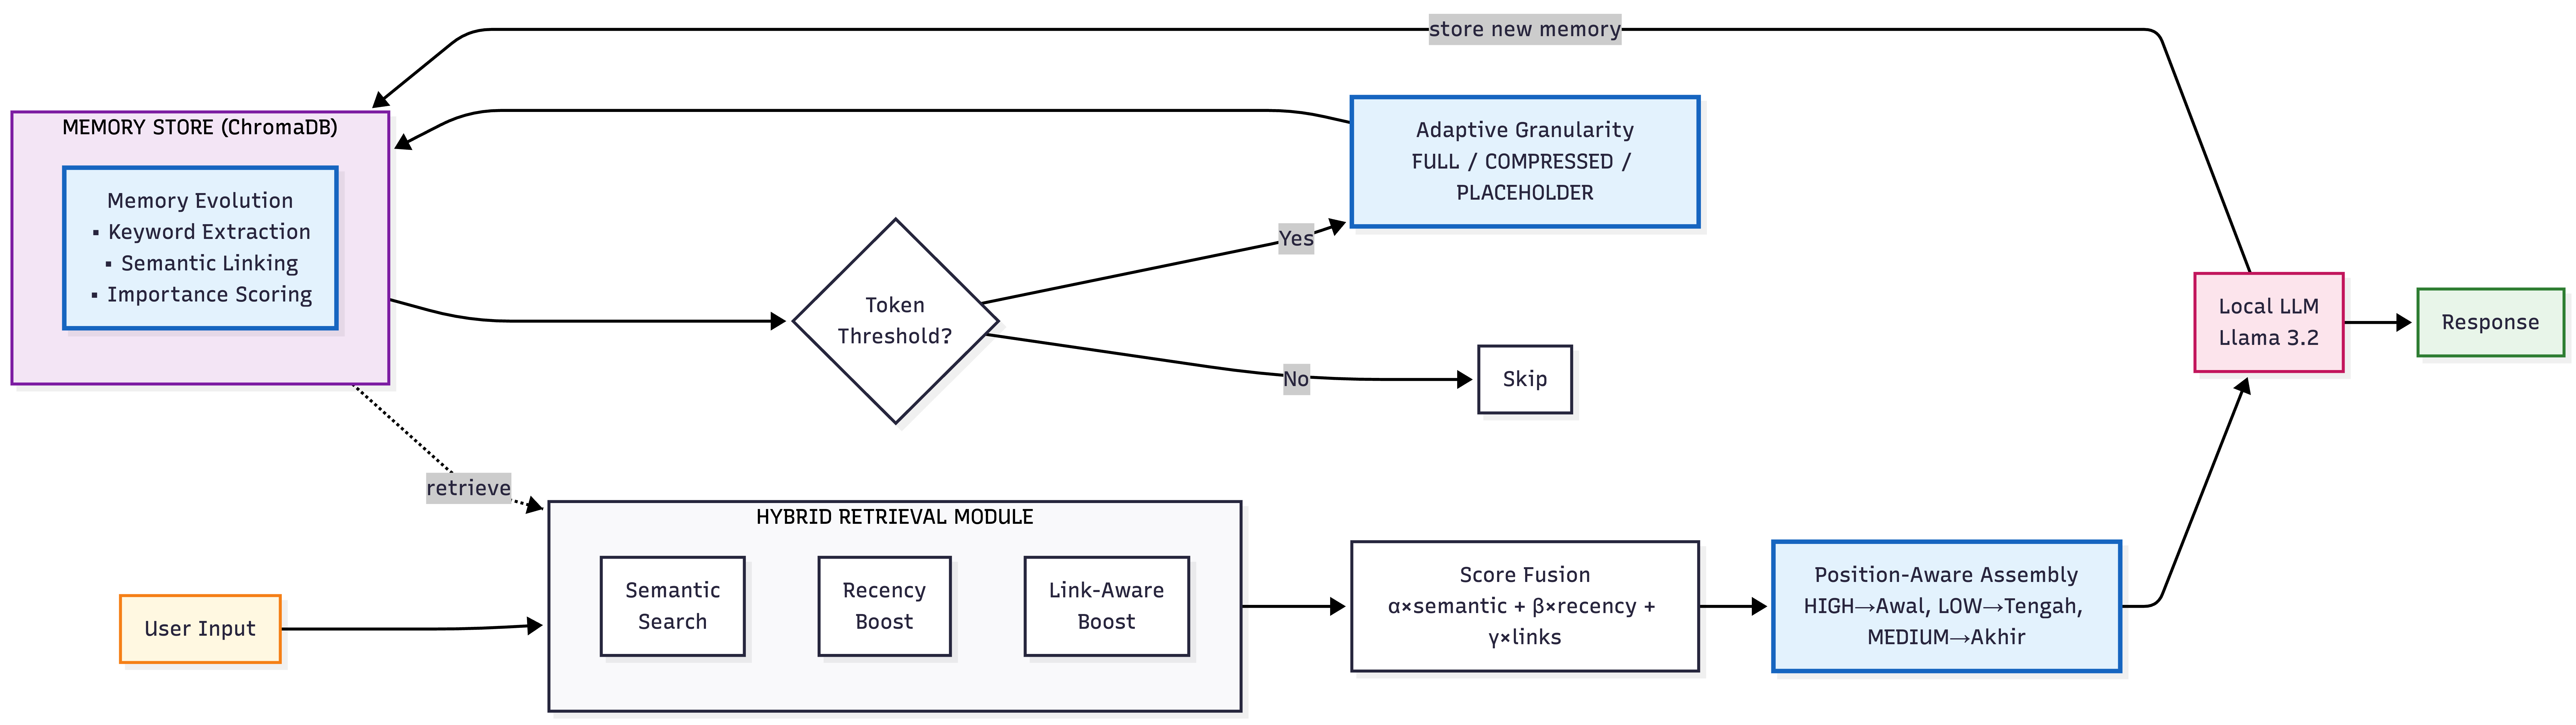
\includegraphics[width=\columnwidth]{fig1.png}}
\caption{The DMF pipeline. A turn is ingested as a \texttt{MemoryChunk}, optionally evolved (keywords, links, importance), retrieved by hybrid scoring, reordered by PA, compressed by AG, and concatenated into the LLM prompt.}
\label{fig:arch}
\end{figure}

\subsection{Memory store}
Each conversational turn becomes a \texttt{MemoryChunk} with a content string, a 384-dimensional embedding produced by \emph{paraphrase-multilingual-MiniLM-L12-v2}, a session and turn identifier, a role tag, a timestamp, and an \texttt{importance\_score} in $[0,2]$. Chunks are persisted in ChromaDB using HNSW with cosine distance.

\subsection{Hybrid retrieval}
Given a query, candidates are scored by
\begin{equation}
\label{eq:hybrid}
\mathrm{score}\;=\;\alpha\cdot \mathrm{sem}\;+\;\beta\cdot \mathrm{rec}\;+\;\gamma\cdot \mathrm{lnk},
\end{equation}
where $\mathrm{sem}$ is cosine similarity, $\mathrm{rec}=e^{-0.1\,d}$ is the Ebbinghaus-style recency factor with $d$ measured in days, and $\mathrm{lnk}$ is an additive contribution from link count and a small connection boost toward the current top-5 semantic matches. The default weights are $(\alpha,\beta,\gamma)=(0.5,0.3,0.2)$; the link term is only active when ME is enabled.

\subsection{Memory Evolution (ME)}
ME builds a semantic graph between memories in three steps. (i)~Keywords are extracted by a term-frequency procedure with an English stop-word list; an LLM-based extractor exists in the implementation but is not used on the evaluation path. (ii)~Bidirectional links are created when the cosine similarity between two memory embeddings exceeds $0.7$, capped at five links per memory. The link type is assigned by a simple heuristic: \texttt{TEMPORAL} when the turn distance is at most 2, \texttt{FOLLOW\_UP} when at most 5, and \texttt{SEMANTIC} otherwise. (iii)~The importance score is updated as
\begin{equation}
\label{eq:importance}
I = 2\,\big(0.30\,r + 0.25\,a + 0.25\,\ell + 0.20\,k\big),
\end{equation}
where $r=2^{-0.01\,h}$ decays exponentially in hours $h$, $a$ is access count normalized by 50, $\ell$ is link count normalized by 10, and $k$ is keyword count normalized by 5. All four components are clipped to $[0,1]$ before the weighted sum so that $I\in[0,2]$.

\subsection{Position-Aware Assembly (PA)}
PA reorders retrieved memories by their normalized importance $\tilde{I}=I/2$. Memories with $\tilde{I}>0.7$ are placed at the beginning of the context to exploit the primacy effect; memories with $\tilde{I}<0.3$ are placed in the middle where attention is weakest; remaining memories are placed at the end to exploit recency. The resulting order is \texttt{[HIGH]\,+\,[LOW]\,+\,[MEDIUM]}. PA reads \texttt{importance\_score} but does \emph{not} compute it; in the absence of ME every memory receives $I=0$, falls into the \texttt{LOW} band, and PA degenerates to the identity. This prerequisite is exploited explicitly in Section~\ref{sec:results} when isolating PA.

\subsection{Adaptive Granularity Summarization (AG)}
AG selects one of three modes for each retrieved memory using both the importance score and the memory age:
\begin{equation}
\label{eq:ag}
\mathrm{mode}(I,h) =
\begin{cases}
\mathrm{DETAILED}    & \text{if } h<24 \;\;\text{or}\;\; I>0.7,\\
\mathrm{COMPRESSED}  & \text{if } h>168 \;\;\text{and}\;\; I<0.3,\\
\mathrm{RAW}         & \text{otherwise.}
\end{cases}
\end{equation}
\texttt{DETAILED} requests an $\sim$80-word LLM summary that preserves names, dates, numbers, and decisions; \texttt{COMPRESSED} requests an $\sim$15-word summary; \texttt{RAW} returns the original text. A safety guard reverts to \texttt{RAW} whenever a generated summary is no shorter than the original text, preventing negative compression.

\section{Implementation and Experimental Setup}
\label{sec:impl}

\textbf{Software stack.} The system is implemented in Python~3.11 with ChromaDB for vector storage, the SentenceTransformers library for embeddings, and Ollama as the LLM runtime. All LLM calls use $\mathrm{temperature}=0$, $\mathrm{seed}=42$, and $\mathrm{top\_p}=1$ for determinism. The evaluation harness caches the ME link graph and the per-query retrieval outputs to JSON on first execution and replays them on subsequent runs, so reported numbers are reproducible from a fresh database.

\textbf{Datasets.} Six custom conversational sessions are used (Table~\ref{tab:sessions}). Each session is annotated with ground-truth memories and multi-hop evaluation queries. Llama 3.2 3B is used for S01--S05; Llama 3.1 8B is used for the S06 large-context boundary study so the LLM is capable of attending to $\sim$10{,}000-token contexts.

\begin{table}[t]
\caption{Session overview}
\label{tab:sessions}
\centering
\renewcommand{\arraystretch}{1.05}
\begin{tabular}{@{}lp{2.7cm}rrrl@{}}
\toprule
\textbf{ID} & \textbf{Domain} & \textbf{Turns} & \textbf{Mem.} & \textbf{Q} & \textbf{Focus} \\
\midrule
S01 & Startup planning      & 60  & 20 & 12 & Ablation \\
S02 & Research coord.       & 80  & 20 & 10 & Ablation \\
S03 & SaaS product dev.     & 70  & 20 & 10 & Ablation \\
S04 & Cloud migration       & 200 & 80 & 12 & PA $K$-sens. \\
S05 & Clinical research     & 100 & 35 & 12 & ME dense-graph \\
S06 & Medical consultation  & 120 & 44 & 12 & PA long context \\
\bottomrule
\end{tabular}
\end{table}

\textbf{Ablation configurations.} Table~\ref{tab:configs} lists the eight configurations. The configuration C5 (\texttt{RAG\_ADAPTIVE\_GRANULARITY} in the codebase) is built on Naive RAG plus AG rather than on Standard RAG plus AG; consequently the comparison C5 vs.\ C2 reflects both the effect of AG and the absence of the recency boost in C5, and the cleanest isolation of AG is C5 vs.\ C1.

\begin{table}[t]
\caption{Ablation configurations}
\label{tab:configs}
\centering
\renewcommand{\arraystretch}{1.05}
\begin{tabular}{@{}clcccl@{}}
\toprule
\textbf{\#} & \textbf{Configuration} & \textbf{ME} & \textbf{PA} & \textbf{AG} & \textbf{Purpose} \\
\midrule
C0 & Base LLM      & --  & --  & --  & Lower bound \\
C1 & Naive RAG     & --  & --  & --  & Simple RAG \\
C2 & Standard RAG  & --  & --  & --  & Baseline \\
C3 & RAG + PA      & --  & \checkmark & --  & Isolate PA \\
C4 & RAG + ME      & \checkmark & --  & --  & Isolate ME \\
C5 & RAG + AG      & --  & --  & \checkmark & Isolate AG \\
C6 & RAG + ME + PA & \checkmark & \checkmark & --  & ME$+$PA interaction \\
C7 & RAG Full      & \checkmark & \checkmark & \checkmark & Full pipeline \\
\bottomrule
\end{tabular}
\end{table}

\textbf{Metrics.} For retrieval we report Precision@$K$, Recall, and F1 against ground-truth memory identifiers. For answer quality (AQ) we use the maximum of a keyword-match score and a token-level F1 score, computed on the LLM output \emph{after} the last ``\#\#\#'' marker; the prompt instructs the model to write its final answer after this marker, and the harness discards any preceding reasoning. For token efficiency (TE) we report the relative reduction in retrieved-context token count due to AG compression.

\textbf{Disclosed evaluation mechanics.} Three implementation details affect every reported number and are stated explicitly. (i)~Each ground-truth memory introduced at turn $T$ is also credited when the retriever returns turn $T{+}1$, since the assistant's confirmation turn typically restates the user's information; this inflates Precision/Recall/F1 relative to a strict single-turn protocol. (ii)~Retrieved candidates whose content overlaps the query by more than 70\% of the shorter length are discarded, and the top-$K$ result list is deduplicated by turn number. (iii)~When AG is enabled, the harness first applies the natural decision logic of~\eqref{eq:ag} and then forces \texttt{COMPRESSED} on every memory not already compressed. This override is necessary because all intra-session memories satisfy the $h<24$~h condition and would otherwise never trigger compression; the reported TE numbers therefore describe an \emph{upper bound} on AG's compression behavior under uniform forcing rather than the natural temporal-adaptive outcome.

\section{Results and Discussion}
\label{sec:results}

\subsection{Main ablation (S01--S03, $K{=}5$)}

Table~\ref{tab:ablation} reports F1, AQ, TE, and the change in F1 relative to the C2 baseline.

\begin{table}[t]
\caption{Ablation study results averaged over S01--S03, $K{=}5$}
\label{tab:ablation}
\centering
\renewcommand{\arraystretch}{1.05}
\begin{tabular}{@{}lcccc@{}}
\toprule
\textbf{Configuration} & \textbf{F1} & \textbf{AQ} & \textbf{TE\,(\%)} & $\boldsymbol{\Delta}$\textbf{F1} \\
\midrule
C0 Base LLM        & 0.000 & 0.173 & 0.0  & --     \\
C1 Naive RAG       & 0.272 & 0.446 & 0.0  & --     \\
C2 Standard RAG    & 0.316 & 0.535 & 0.0  & (base) \\
C3 + PA            & 0.316 & 0.531 & 0.0  & $0.000$  \\
C4 + ME            & 0.310 & 0.508 & 0.0  & $-0.006$ \\
\textbf{C5 + AG}   & \textbf{0.324} & \textbf{0.534} & \textbf{17.7} & $\boldsymbol{+0.008}$ \\
C6 + ME + PA       & 0.219 & 0.373 & 0.0  & $-0.098$ \\
C7 Full DMF        & 0.251 & 0.412 & 16.9 & $-0.065$ \\
\bottomrule
\end{tabular}
\end{table}

C5 (AG only) is the only configuration with a positive $\Delta\mathrm{F1}$ and meaningful TE. Its answer-quality cost is essentially zero ($\Delta\mathrm{AQ}\approx-0.001$ versus C2 and $\approx0$ versus the cleaner C1 baseline). C3 (PA only) is indistinguishable from C2 on every metric, which is expected at $K{=}5$ where the assembled context is far below the Lost-in-the-Middle threshold and PA has at most five chunks to reorder. C4 (ME only) marginally degrades F1 and AQ. The compositions C6 and C7 degrade the F1 of the baseline by 31\% and 21\% respectively; the AG component still produces 16.9\% TE inside C7, indicating that AG's compression is decoupled from the upstream degradation introduced by ME and PA.

\subsection{AG analysis}

AG's positive effect arises because the top-$K$ memories retrieved by hybrid scoring contain substantial redundancy. Adjacent turns often paraphrase the same fact, and the LLM-generated $\sim$15-word summaries retain the salient names and numbers needed to answer the multi-hop queries. The 17.7\% saving is a useful operating point, but two caveats are explicit. First, the saving is measured under the forced-uniform-COMPRESSED override (Section~\ref{sec:impl}); the natural temporal decision of~\eqref{eq:ag} cannot fire on intra-session memories that are uniformly recent. Second, the cleanest comparison is C5 vs.\ C1 because both omit the recency boost; the C5-vs-C2 comparison is reported only for ablation completeness.

\subsection{PA $K$-sensitivity and large-context boundary}

The $\Delta\mathrm{AQ}=0$ in Table~\ref{tab:ablation} could be attributed to insufficient context length. We probe this hypothesis at progressively larger $K$ on S04 (sentence-length memories) and S06 (paragraph-length memories of $\sim$208 tokens each). Table~\ref{tab:pa} shows Recall and $\Delta\mathrm{AQ}$ (RAG~+~ME~+~PA minus RAG~+~ME at the same $K$).

\begin{table}[t]
\caption{PA $K$-sensitivity on S04 and large-context boundary on S06}
\label{tab:pa}
\centering
\renewcommand{\arraystretch}{1.05}
\begin{tabular}{@{}llrrr@{}}
\toprule
\textbf{Session} & \textbf{Setting} & $\boldsymbol{K}$ & \textbf{Recall} & $\boldsymbol{\Delta}$\textbf{AQ} \\
\midrule
S04 & sentences, 3B & 10 & 0.367 & $\phantom{+}0.000$ \\
S04 & sentences, 3B & 20 & 0.575 & $\phantom{+}0.000$ \\
S04 & sentences, 3B & 30 & 0.644 & $+0.009$           \\
S06 & paragraphs, 8B & 20 & 0.638 & $\phantom{+}0.000$ \\
S06 & paragraphs, 8B & 30 & 0.842 & $\phantom{+}0.000$ \\
S06 & paragraphs, 8B & 50 & 0.939 & $\phantom{+}0.000$ \\
\bottomrule
\end{tabular}
\end{table}

On S04, even at $K{=}30$ the assembled context is below $\sim$3{,}000 tokens, so the absence of an effect is consistent with a length-bounded explanation. On S06, however, $K{=}50$ produces an estimated context of $\sim$10{,}383 tokens, exceeding the threshold cited by Liu~\emph{et~al.}~\cite{liu2023lost} above which Lost-in-the-Middle should manifest. PA still produces $\Delta\mathrm{AQ}=0$. Recall rises monotonically with $K$ on both sessions, confirming that the underlying retrieval is functional and that the absence of an effect is not a measurement artifact.

\subsection{Boundary analysis of PA}

Inspection of the importance distribution on S06 explains the result. The clinical-consultation domain is informationally uniform: nearly every paragraph contains a comparable density of named entities, doses, and decisions. ME's importance update therefore produces scores that converge toward a narrow band, and after $\tilde{I}=I/2$ normalization most memories fall into a single PA band. Reordering by a degenerate importance signal cannot help. We further confirm that PA depends on ME upstream: when ME is disabled, every \texttt{importance\_score} is zero, every memory is classified \texttt{LOW}, and PA reduces to the identity function. The diagnostic configuration \texttt{DMF\_PA\_FIXED} in the codebase enables ME solely to populate importance scores while disabling its link-boost; it confirms that PA's true precondition is the \emph{differentiation} of the importance distribution, not the size of the context.

\subsection{ME on dense-entity domains and zero-sum displacement}

S05 was designed to favor ME: the clinical research domain has a dense entity graph (researcher--trial--cohort--outcome--safety-signal) and link expansion should help connect semantically distant but topically relevant memories. Table~\ref{tab:me} reports the comparison.

\begin{table}[t]
\caption{ME on the dense-entity S05 domain, $K{=}5$}
\label{tab:me}
\centering
\renewcommand{\arraystretch}{1.05}
\begin{tabular}{@{}lcccc@{}}
\toprule
\textbf{Approach} & \textbf{P@5} & \textbf{Recall} & \textbf{F1} & \textbf{AQ} \\
\midrule
Standard RAG (C2) & 0.367 & 0.351 & 0.354 & 0.584 \\
DMF + ME          & 0.400 & 0.381 & 0.384 & 0.575 \\
$\Delta$          & $+0.033$ & $+0.030$ & $+0.030$ & $-0.009$ \\
\bottomrule
\end{tabular}
\end{table}

ME does improve retrieval on the dense-entity domain ($\Delta\mathrm{P@5}=+0.033$, $\Delta\mathrm{Recall}=+0.030$), but AQ falls slightly. A per-query breakdown of the 12 evaluation queries reveals the mechanism: 2 queries benefit ($+\mathrm{AQ}$ via link bridges, including a chained \emph{safety signal} retrieval that pure semantic search misses), 2 queries are harmed (a link-expanded memory displaces a directly relevant memory), and the remaining 8 are unchanged. The 17\%/17\%/67\% distribution is characteristic of a \emph{zero-sum displacement} regime: on a fixed $K$, each newly admitted link-expanded memory must evict another. When the displaced memory is more directly relevant than the one that replaces it, AQ falls even as retrieval-set metrics rise. The implication is that link expansion is incompatible with rigid $K$ budgets; an adaptive $K$ or a margin-based admission criterion would be required to extract net benefit on long-form QA.

\subsection{Why composing PA, ME, and AG can degrade performance}

The C6 and C7 results in Table~\ref{tab:ablation} are consistent with the two preceding mechanisms acting in series. ME first reshapes the retrieved set; on $K{=}5$ this trades direct semantic relevance for graph-adjacent material, with a net negative effect. PA then reorders a set that already differs from the optimal one. AG finally compresses the reordered set, but because the upstream selection has degraded, the compression is applied to less relevant content. The full DMF stack inherits the displacement penalty and the lack of importance differentiation simultaneously, producing $\Delta\mathrm{F1}=-0.065$.

\section{Conclusion}
\label{sec:conclusion}

We evaluated three post-retrieval optimizers for LLM conversational memory and found that only the granularity component composes cleanly with a standard hybrid retriever, saving 17.7\% of context tokens with no measurable cost to answer quality under our evaluation regime. The position-aware component shows no effect across all tested context sizes up to $\sim$10{,}383 tokens; its operational bottleneck is the differentiation of the upstream importance distribution, not the length of the context. The memory-evolution component improves retrieval-set metrics on a dense-entity domain but reduces end-to-end answer quality through a zero-sum displacement effect on fixed $K$. Two methodological observations follow: intra-session evaluation cannot exercise the temporal axis of adaptive granularity, and reproducible reporting on memory pipelines requires explicit disclosure of turn-pair retrieval credit, structural answer extraction, and any forced-compression evaluation overrides. Promising directions include LLM-based importance scoring for differentiation, adaptive-$K$ retrieval to mitigate displacement, and multi-session evaluation that exercises the recency axis of compression decisions.

\begin{thebibliography}{99}

\bibitem{liu2023lost}
N.~F. Liu \emph{et~al.}, ``Lost in the middle: How language models use long contexts,'' \emph{Trans.\ Assoc.\ Comput.\ Linguist.}, vol.~12, pp.~157--173, 2024.

\bibitem{lewis2020rag}
P.~Lewis \emph{et~al.}, ``Retrieval-augmented generation for knowledge-intensive NLP tasks,'' in \emph{Adv.\ Neural Inf.\ Process.\ Syst.\ (NeurIPS)}, 2020.

\bibitem{packer2023memgpt}
C.~Packer \emph{et~al.}, ``MemGPT: Towards LLMs as operating systems,'' \emph{arXiv:2310.08560}, 2023.

\bibitem{park2023generative}
J.~S. Park \emph{et~al.}, ``Generative agents: Interactive simulacra of human behavior,'' in \emph{Proc.\ UIST}, 2023.

\bibitem{xu2024amem}
W.~Xu \emph{et~al.}, ``A-MEM: Agentic memory for LLM agents,'' \emph{arXiv:2502.12110}, 2024.

\bibitem{mem0}
Mem0 Team, ``Mem0: The memory layer for personalized AI,'' Tech.\ rep., 2024. [Online]. Available: \url{https://mem0.ai}

\bibitem{cruz2025afm}
A.~Cruz, ``Adaptive fidelity memory for long-running LLM conversations,'' \emph{arXiv preprint}, 2025.

\bibitem{reimers2019sentencebert}
N.~Reimers and I.~Gurevych, ``Sentence-BERT: Sentence embeddings using siamese BERT-networks,'' in \emph{Proc.\ EMNLP-IJCNLP}, 2019, pp.~3982--3992.

\bibitem{touvron2023llama}
H.~Touvron \emph{et~al.}, ``LLaMA: Open and efficient foundation language models,'' \emph{arXiv:2302.13971}, 2023.

\bibitem{ebbinghaus1885}
H.~Ebbinghaus, \emph{\"Uber das Ged\"achtnis: Untersuchungen zur experimentellen Psychologie}. Leipzig: Duncker \& Humblot, 1885.

\bibitem{chroma}
Chroma Development Team, ``Chroma: The AI-native open-source embedding database,'' 2024. [Online]. Available: \url{https://www.trychroma.com}

\bibitem{ollama}
Ollama Project, ``Ollama: Run large language models locally,'' 2024. [Online]. Available: \url{https://ollama.com}

\end{thebibliography}

\end{document}
